\documentclass[12pt]{article}
\usepackage[utf8]{inputenc}
\usepackage[T1]{fontenc}
\usepackage{lmodern}
\usepackage{setspace}
\usepackage{geometry}
\usepackage{url}
\usepackage{graphicx}

\geometry{
  left=1in,
  right=1in,
  top=1in,
  bottom=1in
}

\begin{document}

%-------------------------------
%           TITLE PAGE
%-------------------------------
\begin{titlepage}
\begin{center}

{\Large \textbf{ASL Recognition System:\\[6pt] Bridging Gaps in Communication Accessibility}}\\[2cm]

{\normalsize A Thesis Submitted in partial fulfillment of the Requirements of the\\
Renée Crown University Honors Program at Syracuse University}\\[1.5cm]

{\large \textbf{Carlo F. Pisacane}}\\[0.5cm]
{\normalsize Candidate for Bachelor’s of Science in Computer Science\\
and Renée Crown University Honors\\
May 2025}\\[3cm]

{\Large \textbf{Honors Thesis in Computer Science}}\\[1.5cm]
\begin{tabbing}
\hspace*{3cm}\= \kill
Thesis Advisor:\> \underline{\hspace{4cm}} \\
\> Dr.\ Nadeem Ghani, Assistant Teaching Professor\\[1cm]
Thesis Reader:\> \underline{\hspace{4cm}} \\
\> Dr.\ João Paulo Marum, Assistant Teaching Professor\\[1cm]
Honors Director:\> \underline{\hspace{4cm}} \\
\> Dr.\ Danielle Smith, Director
\end{tabbing}
\vfill

\end{center}
\end{titlepage}

\clearpage
\pagenumbering{roman}
\setcounter{page}{1}
\pagestyle{plain}


\newpage
\vspace*{\fill}        
\begin{center}
    {\small © Syracuse University 2025. All rights Reserved}
\end{center}
\vspace*{\fill}
\newpage

%-------------------------------
%           ABSTRACT
%-------------------------------
\clearpage
\section*{Abstract}
\vspace{1em}

\noindent
A concise summary of your research, covering the problem (gaps in existing ASL recognition 
systems), your proposed solution (ASL recognition tool), methodology, key findings, and
conclusions. 

\vspace{2em}
\noindent
\textbf{Thesis Advisor:} Nadeem Ghani \\
\textbf{Title:} Assistant Teaching Professor, Engineering and Computer Science

%-------------------------------
%       ACKNOWLEDGMENTS
%-------------------------------
\newpage
\doublespacing
\section*{Acknowledgments}

I am deeply grateful for the support and guidance I have received throughout my academic journey at Syracuse University. I would like to extend my sincere thanks to my advisor, Prof. Nadeem Ghani, whose mentorship was instrumental in shaping my research and academic pursuits. My gratitude also goes to my thesis reader, Prof. João Marum, for his valuable insights and constructive feedback.

I am particularly thankful to Robin Smith, my Honors advisor, for motivating and encouraging me over the past four years during my time in the Honors program and throughout the thesis development process. Their support helped me overcome challenges and remain focused on my goals.

Finally, I am forever indebted to my friends and family, whose encouragement and belief in me have been a constant source of inspiration.


%-------------------------------
%       Preface
%-------------------------------
\newpage
\doublespacing
\section*{Preface}

Why I chose this topic, personal insights, and what I learned, reference: CS example 
thesis.pdf (Kyle Maiorana)

\clearpage
\pagenumbering{arabic}
\setcounter{page}{1}
\doublespacing

%-------------------------------
%     TABLE OF CONTENTS
%-------------------------------
\newpage
\tableofcontents
\newpage

%-------------------------------
%     LIST OF FIGURES
%-------------------------------
\listoffigures
\newpage

%-------------------------------
%   CHAPTER 1 / INTRODUCTION
%-------------------------------
\doublespacing

\newpage
\section*{Chapter 1}
\addcontentsline{toc}{section}{Chapter 1}
\begin{center}
\large \textbf{Introduction}
\end{center}

Communication is a fundamental human need, and for Deaf and hard-of-hearing individuals, 
American Sign Language (ASL) serves as a primary mode of expression. ASL is a rich and 
complex visual language based on hand shape, movement, and nonmanual markers such as facial 
expressions. Studies emphasizing Deaf-centric design have shown that effective ASL tools must 
respect the cultural and linguistic practices of the Deaf community (Hibbard et al., 2020 [1]).

Technology has evolved from the past to make communication more accessible, including captioning 
services, text-based messaging, and video relay services. However, these solutions often rely on 
real-time interpreters or a shared written language, which can be limiting in spontaneous, in-person 
conversations.

In recent years, advances in computer vision and machine learning have opened new 
avenues for automated sign language recognition. Leveraging the power of advanced algorithms 
and increasingly pervasive hardware (e.g., mobile phone cameras, webcams), engineers and 
researchers hope to create machines that can recognize ASL hand gestures in real time. While 
some progress has been made in recognizing static signs or alphabets (Debnath and Joe, 2024 [3]), 
challenges remain, especially regarding vocabulary expansion, nonmanual features, and real-world 
performance (Falvo et al., 2020 [2]). The present work focuses on addressing these challenges by 
developing a user-centered ASL recognition tool that emphasizes accuracy, speed, and accessibility.

\vspace{1.5em}
\noindent
\textbf{1.1 Research Problem}
\addcontentsline{toc}{subsection}{1.1 Research Problem}
\vspace{1.5em}

Current ASL recognition systems have several limitations that make them impractical. Some systems 
recognize only a limited set of signs, which restricts real-world applicability. Others do not 
account for nonmanual signs, such as facial expressions or head tilts, which are essential in ASL 
for the expression of tone, grammatical markers, and emotional context. Additionally, some tools 
demand specialized sensors that are expensive or inconvenient, thus deterring widespread use.

There is also a broad gap in designing user interfaces that are responsive to the needs and desires 
of Deaf individuals. Inaccurate calibration procedures, variability of performance under changing 
lighting conditions, or excessive latency can lower the usability of a system. These barriers 
compound to inhibit the real-world deployment potential of ASL recognition technology in everyday 
communication (Falvo et al., 2020 [2]).

\vspace{1.5em}
\noindent
\textbf{1.2 Research Objectives}
\addcontentsline{toc}{subsection}{1.2 Research Objectives}
\vspace{1.5em}

The overall goal of this thesis is to design a real-time ASL recognition system using computer 
vision and machine learning techniques. Specifically, the system must offer high recognition 
accuracy. The second aim is to enhance user experience by developing an accessible interface that 
is easy to install and requires minimal calibration or dedicated hardware. Additionally, the system 
needs better performance in the range of lighting and backgrounds found in real world environments. Finally, the framework needs to be extensible 
for future additions of other signs, dynamic gestures, and nonmanual signals. By focusing on these 
core objectives, the system aims to be a foundation for broader applications in education, assistive 
technology, and inclusive communication devices.

\vspace{1.5em}
\noindent
\textbf{1.3 Significance of the Study}
\addcontentsline{toc}{subsection}{1.3 Significance of the Study}
\vspace{1.5em}

This project holds the potential for shattering communication barriers among the Deaf and 
hard-of-hearing and for providing meaningful resources for hearing individuals who wish to learn 
ASL. An effective real-time ASL recognition system can facilitate communication more effectively 
in public places, schools, and workplaces, particularly where access to interpreters may not be 
readily available. It can also serve as an interactive learning tool for ASL learners, offering 
instant feedback on handshapes to facilitate language learning. The proposed framework can further 
be extended to encompass the full richness of sign languages, thereby enabling future research 
studies. By prioritizing usability and involving Deaf/ASL communities in the design, this research 
underscores the importance of user-centered solutions.

\vspace{1.5em}
\noindent
\textbf{1.4 Thesis Structure}
\addcontentsline{toc}{subsection}{1.4 Thesis Structure}
\noindent
This thesis is organized into five main chapters:

\begin{enumerate}
  \item \textbf{Chapter 1: Introduction}\\
  Provides the background and context of ASL recognition, defines the research problem, outlines objectives, and explains the study’s significance.
  \item \textbf{Chapter 2: Literature Review}\\
  Examines existing ASL recognition systems, machine learning techniques, and user-centered design principles. Identifies gaps in the current research and sets the stage for the proposed approach.
  \item \textbf{Chapter 3: Software and Application}\\
  Details the methodology, including data collection, model architecture, and real-time inference pipeline. Discusses the design choices and rationale behind the system’s implementation.
  \item \textbf{Chapter 4: Results}\\
  Presents empirical findings, including model performance metrics, real-time testing results, and user feedback. Analyzes both quantitative and qualitative data.
  \item \textbf{Chapter 5: Conclusion}\\
  Summarizes key insights, highlights contributions, and suggests avenues for future work. Reflects on the system’s potential impact on accessibility and communication technologies.
\end{enumerate}

%-------------------------------
%   CHAPTER 2 / Literature Review
%-------------------------------
\newpage
\section*{Chapter 2}
\addcontentsline{toc}{section}{Chapter 2}
\begin{center}
    \large \textbf{Literature Review}
\end{center}

\vspace{1.5em}
\noindent
\textbf{2.1 Introduction}
\addcontentsline{toc}{subsection}{2.1 Introduction}
\vspace{1em}

This literature review surveys various methods and technologies employed in American 
Sign Language (ASL) recognition systems. The goal is to establish how our approach, aimed 
at real-time recognition and user-friendly interaction fits into the existing body of work.
By examining both hardware-based and vision-based solutions, we highlight the fundamental 
challenges and opportunities in creating accessible tools for Deaf and hard-of-hearing 
communities.

\vspace{1.5em}
\noindent
\textbf{2.2 Overview of Existing ASL Recognition Systems}
\addcontentsline{toc}{subsection}{2.2 Overview of Existing ASL Recognition Systems}
\vspace{1em}

Recent developments in sign language recognition often revolve around three main 
technological streams:

\begin{itemize}
    \item Computer Vision Approaches
    \item Depth Sensor Approaches
    \item Wearable Technology Approaches
\end{itemize}

Each of these streams has strengths and limitations related to cost, accuracy, ease of 
deployment, and user comfort. This section reviews notable research in these areas and 
provides the groundwork for our own system’s design choices.

\vspace{1.0em}
\noindent
\textbf{2.2.1 Computer Vision Approaches}
\addcontentsline{toc}{subsubsection}{2.2.1 Computer Vision Approaches}
\vspace{0.5em}

A substantial portion of ASL recognition research leverages standard RGB cameras and 
a variety of computer vision techniques. Traditional pipelines often involve skin detection, 
feature extraction, and hand segmentation before proceeding to classification. More recently, 
robust libraries like \textit{OpenCV} and frameworks such as \textit{MediaPipe} have significantly simplified 
and improved hand detection and tracking.

One notable example is the \textit{MediaPipe Hands} solution, an open-source tool by Google\footnote{\url{https://github.com/google-ai-edge/mediapipe/blob/master/docs/solutions/hands.md}}. 
MediaPipe Hands tracks 21 key landmarks on each hand, as illustrated in Figure~\ref{fig:mediapipe_hands}. This 
framework provides real-time tracking even under challenging conditions such as varied lighting 
or partial occlusions, which is crucial for the fluid and rapid gestures of sign language.

\begin{figure}[h!]
  \centering
  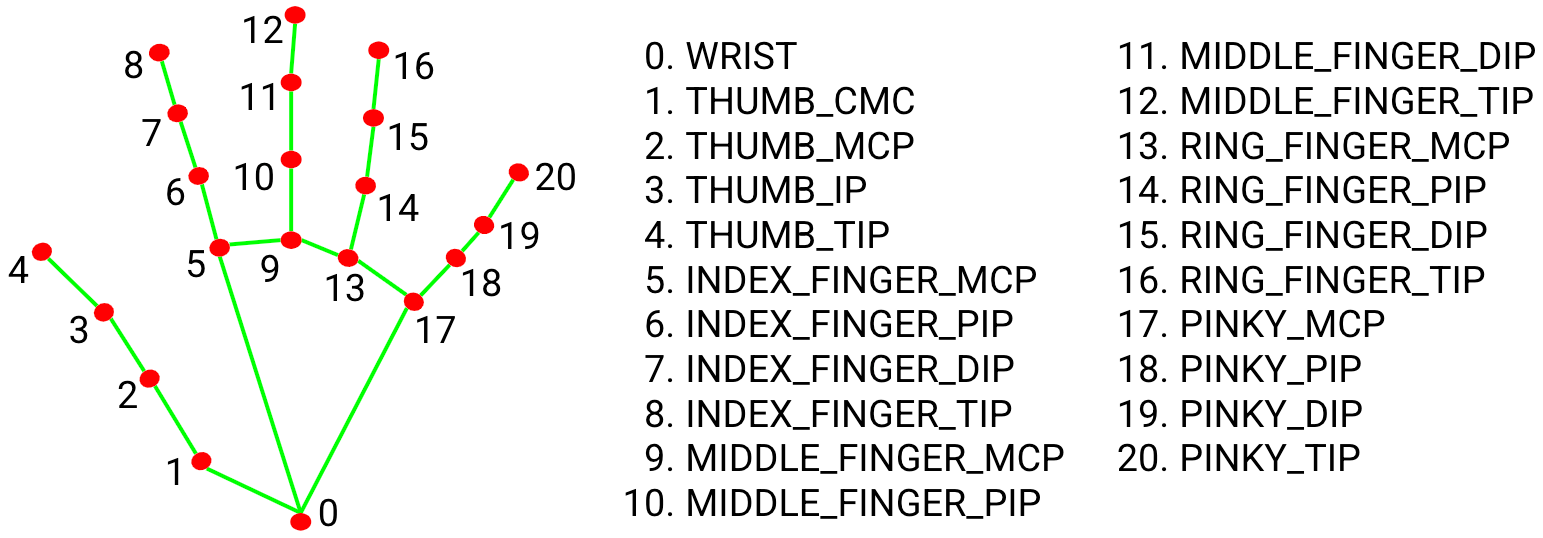
\includegraphics[width=0.95\textwidth]{MediaPipe_hands.png}
  \caption{MediaPipe Hands landmarks. Each point corresponds to a specific joint or fingertip.}
  \label{fig:mediapipe_hands}
\end{figure}

Researchers have successfully integrated MediaPipe’s tracking features into sign language 
systems to reduce the complexity of manual feature engineering. For instance, Debnath and 
Joe~\cite{ref3} demonstrate a real-time ASL detection setup where MediaPipe is employed to extract 
hand pose information, thereby reliably differentiating between common ASL hand shapes 
and movements.

\vspace{1.0em}
\noindent
\textbf{2.2.2 Depth Sensor Approaches}
\addcontentsline{toc}{subsubsection}{2.2.2 Depth Sensor Approaches}
\vspace{0.5em}

Beyond standard RGB cameras, \textit{depth sensors} capture three-dimensional information 
about hand positions. Notably, Avola et al.~\cite{ref4} illustrate how the Leap Motion Controller 
can track the skeletal structure of the hand with fine-grained accuracy, enabling precise 
measurement of joint angles. This capability is beneficial for distinguishing 
similar signs that differ only slightly in finger placement or orientation.

\vspace{1.0em}
\noindent
\textbf{2.2.3 Wearable Technology Approaches}
\addcontentsline{toc}{subsubsection}{2.2.3 Wearable Technology Approaches}
\vspace{0.5em}

Finally, some research efforts rely on \textit{wearable devices}, such as glove-based sensors, to 
record hand movements. These systems, often equipped with inertial measurement units 
(IMUs) or bend sensors, can capture motion data in three dimensions. For example, 
Stefanidis et al.~\cite{ref5} discuss the use of 3D technologies in sign language applications 
through wearable platforms. While potentially more accurate, such devices can be costly or 
cumbersome, limiting their broad adoption for everyday use.

\vspace{1.5em}
\noindent
\textbf{2.3 Summary}
\addcontentsline{toc}{subsection}{2.3 Summary}
\vspace{1em}

In summary, contemporary ASL recognition solutions range from purely vision-based 
approaches (e.g., MediaPipe Hands combined with OpenCV for live detection) to more 
specialized hardware solutions (e.g., depth sensors and wearable gloves). Among these, live 
vision-based detection using MediaPipe and OpenCV offers the optimal balance of high 
accuracy, cost-effectiveness, and ease of integration, making it the best choice for designing 
robust, real-time ASL recognition systems that can be easily adopted in real-world contexts.

%-------------------------------------------
%   2.4 MACHINE LEARNING APPROACHES FOR GESTURE RECOGNITION
%-------------------------------------------

\vspace{1.5em}
\noindent
\textbf{2.4 Machine Learning Approaches for Gesture Recognition}
\addcontentsline{toc}{subsection}{2.4 Machine Learning Approaches for Gesture Recognition}
\vspace{1em}

Advances in deep learning have been essential in enhancing sign language recognition 
by addressing both spatial and temporal complexities. In our work and as demonstrated in 
previous studies (Papastratis et al., 2021 [9] and Ru and Sebastian, 2023 [10]), a combination 
of Convolutional Neural Networks (CNNs), Recurrent Neural Networks (RNNs), and Long 
Short-Term Memory (LSTM) networks has been used to capture static hand features as well 
as the dynamic information inherent in continuous gestures.

\vspace{1em}
\noindent
\textbf{2.4.1 Convolutional Neural Networks (CNNs) for Static Sign Recognition}
\addcontentsline{toc}{subsubsection}{2.4.1 Convolutional Neural Networks (CNNs) for Static Sign Recognition}
\vspace{1em}

CNNs excel at extracting spatial features from images or individual video frames. 
Their layered architecture enables the learning of hierarchical representations that can 
effectively distinguish subtle differences in hand shape and orientation. In the context of ASL 
recognition, CNNs have been successfully used to classify isolated, static signs before further 
processing is applied (Debnath and Joe, 2024 [3]).

% \begin{figure}[h!]
%   \centering
%   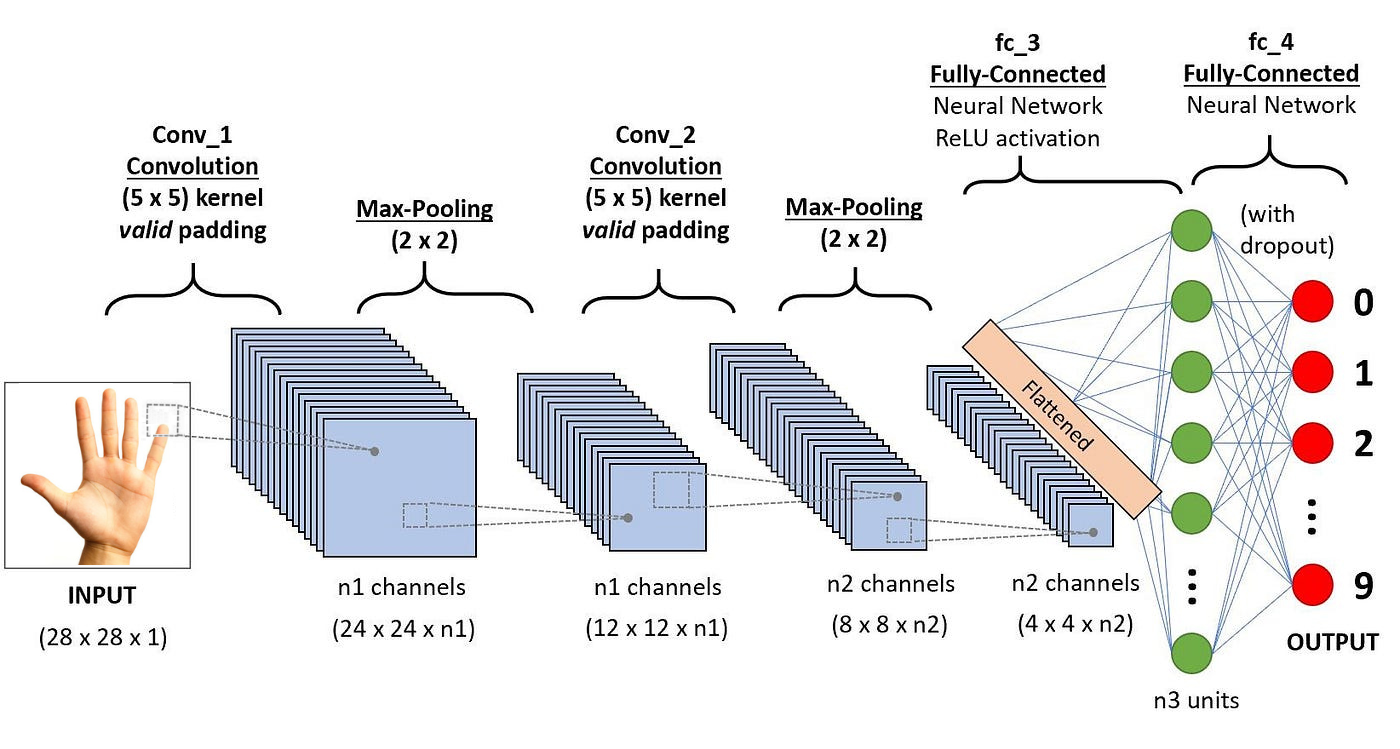
\includegraphics[width=0.95\textwidth]{cnn_architecture.png}
%   \caption{An illustration of a CNN architecture depicting convolutional layers, pooling layers, and fully connected layers, highlighting the extraction of features from a hand image.}
%   \label{fig:cnn_architecture}
% \end{figure}

\vspace{1em}
\noindent
\textbf{2.4.2 Recurrent Neural Networks (RNNs) and Long Short-Term Memory (LSTMs) for Dynamic Sign Recognition}
\addcontentsline{toc}{subsubsection}{2.4.2 Recurrent Neural Networks (RNNs) and LSTMs for Dynamic Sign Recognition}
\vspace{1em}

Dynamic signs which involve motion and transitions require models that can capture 
temporal dependencies. Traditional RNNs are naturally suited for sequential data, but 
they often encounter difficulties when processing long input sequences 
(Avola et al., 2019 [4]; Liu et al., 2016 [6]). LSTM networks, introduced to overcome these 
limitations, incorporate memory cells and gating mechanisms that enable them to retain 
and update information over extended periods (Hochreiter and Schmidhuber, 1997 [7]; Colah’s 
Blog, 2015 [8]). These capabilities make LSTMs particularly effective for recognizing 
continuous ASL gestures.

% \begin{figure}[h!]
%   \centering
%   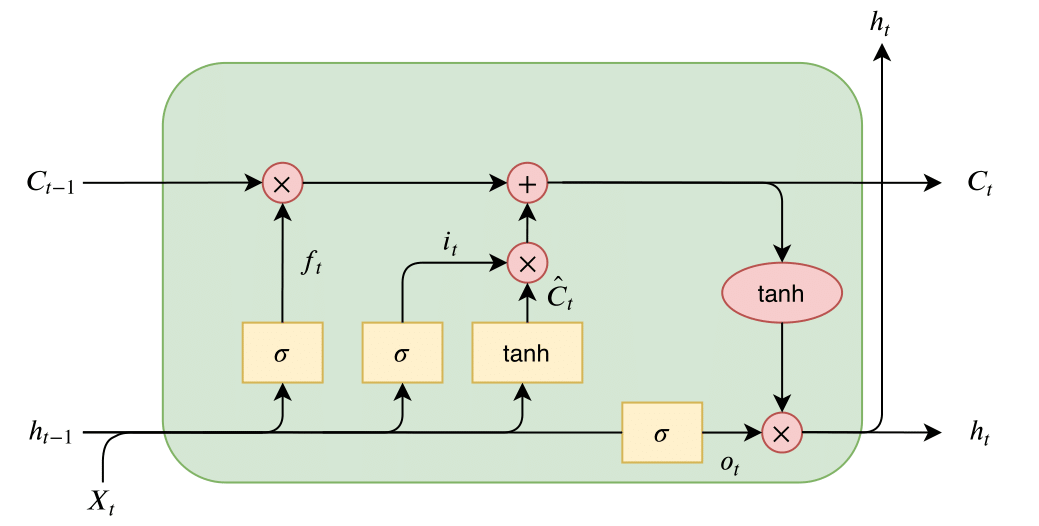
\includegraphics[width=0.85\textwidth]{lstm_architecture.png}
%   \caption{A diagram showing the internal structure of an LSTM cell—including input, forget, and output gates—and an unrolled LSTM network across a sequence of video frames.}
%   \label{fig:lstm_architecture}
% \end{figure}

Hybrid architectures that combine CNNs and LSTMs have also proven effective. In 
such systems, CNNs first extract deep features from each frame, and these features are 
then processed by LSTMs to capture the sequential dynamics of the gesture (Papastratis 
et al., 2021 [9]; Ru and Sebastian, 2023 [10]). This two-stage approach enhances accuracy, 
particularly in real-world scenarios where both spatial and temporal information are crucial.

\vspace{1em}
\noindent
\textbf{2.4.3 Handling Static vs. Dynamic Signs}
\addcontentsline{toc}{subsubsection}{2.4.3 Handling Static vs. Dynamic Signs}
\vspace{1em}

The choice of model architecture is dictated by the nature of the sign:
\begin{itemize}
    \item \textbf{Static Signs:} When the sign consists of a fixed hand posture, CNNs can be employed 
    alone to capture the necessary spatial features.
    \item \textbf{Dynamic Signs:} For gestures that involve motion, models such as RNNs and, more 
    effectively, LSTMs are essential. Their ability to model long-term dependencies allows 
    them to interpret the temporal evolution of a gesture accurately. Many systems adopt 
    a two-stage approach, first applying CNNs for frame-wise feature extraction, followed 
    by LSTMs to model the sequential aspects of the gesture (Lee et al., 2021 [11]).
\end{itemize}

\vspace{1em}
\noindent
\textbf{2.4.4 Integration of Recursive Neural Network Approaches}
\addcontentsline{toc}{subsubsection}{2.4.4 Integration of Recursive Neural Network Approaches}
\vspace{1em}

Recent work has also explored recursive neural network architectures for capturing hierarchical 
structures in sign language gestures (Borges-Galindo et al., 2024 [12]). Although 
our primary focus is on CNN-LSTM hybrids, recursive models offer a promising alternative 
for handling complex information in gestures and may be considered for future 
extensions of our system.

%-------------------------------------------
%   2.5 BASE REPOSITORY FOR IMPLEMENTATION
%-------------------------------------------

\vspace{1.5em}
\noindent
\textbf{2.5 Base Repository for Implementation}
\addcontentsline{toc}{subsection}{2.5 Base Repository for Implementation}
\vspace{1em}

Our ASL recognition system builds upon the open-source repository by K. Takahashi, 
“hand-gesture-recognition-mediapipe” [13]. This repository provides a robust baseline that 
leverages the MediaPipe library for real-time hand and body landmark detection. By integrating 
MediaPipe’s efficient tracking algorithms with our CNN-LSTM architecture, our 
system extracts key spatial features and processes them in real time for accurate gesture 
recognition.

% \begin{figure}[h!]
%   \centering
%   \includegraphics[width=0.8\textwidth]{system_pipeline.png}
%   \caption{A block diagram depicting the overall system pipeline—from video capture and MediaPipe-based landmark extraction to CNN-based feature extraction and LSTM-based temporal classification.}
%   \label{fig:system_pipeline}
% \end{figure}

This base repository has been instrumental in our progress, enabling rapid prototyping 
and rigorous testing under real-world conditions.

%-------------------------------------------
%   2.6 CHALLENGES AND GAPS IN CURRENT SYSTEMS
%-------------------------------------------

\vspace{1.5em}
\noindent
\textbf{2.6 Challenges and Gaps in Current Systems}
\addcontentsline{toc}{subsection}{2.6 Challenges and Gaps in Current Systems}
\vspace{1em}

Despite significant advances in ASL recognition technologies, several critical challenges 
and gaps remain that hinder widespread adoption in real-world settings:

\begin{itemize}
    \item \textbf{Limited Vocabulary and Generalization:}  
    Many existing systems are designed to recognize only a restricted set of signs, 
    making it difficult to scale to larger vocabularies. This limitation often stems 
    from insufficient training data and models that are tuned for a narrow set of gestures 
    (Debnath and Joe, 2024 [3]). Consequently, these systems struggle to generalize across 
    different signers or adapt to variations in signing styles.

    \item \textbf{Difficulty Capturing Nonmanual Signals:}  
    Effective sign language communication relies not only on hand gestures but also on 
    nonmanual signals such as facial expressions and head tilts. Current approaches often 
    neglect these critical features due to the complexities involved in accurately capturing 
    and processing them. As a result, essential grammatical and emotional nuances are frequently 
    lost, limiting the overall accuracy and naturalness of the interpretation 
    (Avola et al., 2019 [4]).

    \item \textbf{Poor Performance in Real-World Environments:}  
    Many systems demonstrate high accuracy under controlled conditions; however, 
    performance typically degrades in real-world scenarios. Factors such as variable lighting 
    conditions, dynamic backgrounds, and ambient noise can adversely affect both the feature
    extraction process and the robustness of the model (Liu et al., 2016 [6]). These challenges 
    underscore the need for systems that maintain high performance in diverse and unpredictable 
    environments.

    \item \textbf{User Interface and Accessibility Shortcomings:}  
    Beyond the technical aspects of recognition, user experience plays a pivotal role in 
    the adoption of ASL systems. Current implementations often suffer from complex calibration 
    procedures, unintuitive interfaces, or hardware requirements that are not easily accessible 
    to the Deaf community. Such issues can discourage user engagement and limit the practical 
    utility of the technology (Hibbard et al., 2020 [1]).
\end{itemize}

%-------------------------------------------
%   2.7 CONCLUSION
%-------------------------------------------

\vspace{1.5em}
\noindent
\textbf{2.7 Conclusion}
\addcontentsline{toc}{subsection}{2.7 Conclusion}
\vspace{1em}

In summary, while state-of-the-art ASL recognition systems have made commendable 
progress, significant gaps remain, particularly in vocabulary generalization, the integration of 
nonmanual signals, robustness in real-world conditions, and user accessibility. Our proposed 
system addresses these issues by leveraging a hybrid CNN-LSTM architecture integrated with 
MediaPipe for real-time, robust hand and body landmark detection. By focusing on 
a user-centered design and optimizing performance under varying environmental conditions, 
the system aims to offer:

\begin{itemize}
    \item \textbf{Real-Time Performance:}  
    Ensuring quick and accurate recognition through efficient deep learning models and 
    streamlined data processing pipelines.
    
    \item \textbf{Robust Detection:}  
    Enhancing accuracy across a wide range of signs, including both manual and nonmanual 
    signals, by employing advanced feature extraction and temporal modeling techniques.
    
    \item \textbf{User-Friendly Interface:}  
    Prioritizing accessibility and ease of use, with minimal calibration requirements and 
    an intuitive design that caters to the needs of Deaf and hard-of-hearing individuals.
\end{itemize}

This conclusion sets the stage for the subsequent methodology chapter, where we will 
detail the system architecture, data acquisition procedures, and the experimental protocols 
implemented to validate our approach.

%-------------------------------
%   CHAPTER 3 / Software and Application
%-------------------------------
\newpage
\section*{Chapter 3}
\addcontentsline{toc}{section}{Chapter 3}
\begin{center}
\large \textbf{Software and Application}
\end{center}

Include text here

\vspace{1.5em}
\noindent
\textbf{3.1 }
\addcontentsline{toc}{subsection}{3.1}
\vspace{1.5em}

Include text here

%-------------------------------
%   CHAPTER 4 / Results (Analysis)
%-------------------------------
\newpage
\section*{Chapter 4}
\addcontentsline{toc}{section}{Chapter 4}
\begin{center}
\large \textbf{Results}
\end{center}

Include text here

\vspace{1.5em}
\noindent
\textbf{4.1 }
\addcontentsline{toc}{subsection}{4.1}
\vspace{1.5em}

Include text here

%-------------------------------
%   CHAPTER 5 / Conclusion
%-------------------------------
\newpage
\section*{Chapter 5}
\addcontentsline{toc}{section}{Chapter 5}
\begin{center}
\large \textbf{Conclusion}
\end{center}

Include text here

\vspace{1.5em}
\noindent
\textbf{5.1 }
\addcontentsline{toc}{subsection}{5.1}
\vspace{1.5em}

Include text here

%-------------------------------
%   BIBLIOGRAPHY
%-------------------------------
\clearpage
\onehalfspacing

\renewcommand{\refname}{Bibliography}
\addcontentsline{toc}{section}{Bibliography}

\begin{thebibliography}{99}

% TerpTube
\bibitem{ref1}
E.~Hibbard \emph{et al.}, 
“Getting a Sign in Edgewise: User-Centered Design Considerations in Creating a Signed Language Mentoring Management System,” 
\emph{Sign Language Studies}, vol.~20, no.~2, pp.~264--300, 2020. 
Available: \url{https://www.jstor.org/stable/26983963}  

% Deaf info
\bibitem{ref2}
V. Falvo, L. P. Scatalon, and E. F. Barbosa, 
“The Role of Technology to Teaching and Learning Sign Languages: A Systematic Mapping,” 
in \emph{2020 IEEE Frontiers in Education Conference (FIE)}, Uppsala, Sweden, 2020, pp.~1--9, 
doi: \texttt{10.1109/FIE44824.2020.9274169}.  
Available: \url{https://ieeexplore-ieee-org.libezproxy2.syr.edu/document/9274169}

% OpenCV, MediaPipe, LSTMs 
\bibitem{ref3}
J.~Debnath and P.~J.~I R, 
“Real-Time Gesture Based Sign Language Recognition System,” 
in \emph{2024 International Conference on Advances in Data Engineering and Intelligent Computing Systems (ADICS)}, 
Chennai, India, 2024, pp.~01--06, 
doi: \texttt{10.1109/ADICS58448.2024.10533518}.
Available: \url{https://ieeexplore-ieee-org.libezproxy2.syr.edu/document/10533518}

% Leap motion sensor + LSTMs
\bibitem{ref4}
D.~Avola, M.~Bernardi, L.~Cinque, G.~L.~Foresti, and C.~Massaroni, 
“Exploiting Recurrent Neural Networks and Leap Motion Controller for the Recognition of Sign Language and Semaphoric Hand Gestures,” 
\emph{IEEE Transactions on Multimedia}, vol.~21, no.~1, pp.~234--245, Jan.~2019, 
doi: \texttt{10.1109/TMM.2018.2856094}. 
Available: \url{https://ieeexplore.ieee.org/document/8410764}

% Gloves and different wearable technologies
\bibitem{ref5}
Stefanidis, Kiriakos, Dimitrios Konstantinidis, Thanassis Kalvourtzis,  
Kosmas Dimitropoulos, and Petros Daras.  
“3D technologies and applications in sign language.” 2020. 
Available: \url{https://www.researchgate.net/publication/340966069_3D_technologies_and_applications_in_sign_language}

% LSTMs
\bibitem{ref6}
T.~Liu, W.~Zhou, and H.~Li, 
“Sign language recognition with long short-term memory,” 
in \emph{2016 IEEE International Conference on Image Processing (ICIP)}, 
Phoenix, AZ, USA, 2016, pp.~2871--2875, 
doi: \texttt{10.1109/ICIP.2016.7532884}.  
Available: \url{https://ieeexplore-ieee-org.libezproxy2.syr.edu/document/7532884}

% LSTM textbook
\bibitem{ref7}
S.~Hochreiter and J.~Schmidhuber, 
“Long Short-Term Memory,” 
in \emph{Neural Computation}, vol.~9, no.~8, pp.~1735--1780, Nov.~15, 1997, 
doi: \texttt{10.1162/neco.1997.9.8.1735}. 
Available: \url{https://ieeexplore.ieee.org/document/6795963}

% Learn LSTMs
\bibitem{ref8}
C. Olah, 
“Understanding LSTM Networks,” 
Understanding LSTM Networks, Aug. 17, 2015. [Online].  
Available: \url{https://colah.github.io/posts/2015-08-Understanding-LSTMs/}

\bibitem{ref9}
I.~Papastratis \emph{et al.}, 
“Artificial Intelligence Technologies for Sign Language,” 
\emph{Sensors (Basel, Switzerland)}, vol.~21, no.~17, p.~5843, Aug.~30, 2021, 
doi: \texttt{10.3390/s21175843}.   
Available: \url{https://pmc.ncbi.nlm.nih.gov/articles/PMC8434597/}

% CNNs LSTMs
\bibitem{ref10}
J.~T.~S. Ru and P. Sebastian, 
“Real-Time American Sign Language (ASL) Interpretation,” 
in \emph{2023 2nd International Conference on Vision Towards Emerging Trends in Communication and Networking Technologies (ViTECoN)}, 
Vellore, India, 2023, pp.~1--6, 
doi: \texttt{10.1109/ViTECoN58111.2023.10157157}. 
Available: \url{https://ieeexplore-ieee-org.libezproxy2.syr.edu/document/10157157}

% RNNs and LSTMs 
\bibitem{ref11}
C.~K.~M. Lee, K.~K.~H. Ng, C.-H. Chen, H.~C.~W. Lau, S.~Y. Chung, and T. Tsoi, 
“American sign language recognition and training method with recurrent neural network,” 
\textit{Expert Systems with Applications}, vol.~167, pp.~114403, 2021,  
ISSN 0957-4174.  
Available: \url{https://doi.org/10.1016/j.eswa.2020.114403} 

% MSL (CLSTM / LSTM / RNN) MEDIAPIPE, OPENCV *PROF REC*
\bibitem{ref12}
E.~A. Borges-Galindo \emph{et al.}, 
“Sign Language Interpreting System Using Recursive Neural Networks,” 
\emph{Applied Sciences}, vol.~14, no.~18, Art. no. 8560, Sep.~23, 2024,  
Available: \url{https://www.mdpi.com/2076-3417/14/18/8560}

% original project
\bibitem{ref13}
K. Takahashi, “hand-gesture-recognition-mediapipe,” GitHub repository,  
Available: \url{https://github.com/kinivi/hand-gesture-recognition-mediapipe} (Accessed: Feb. 26, 2025)

% % Keras textbook
% \bibitem{ref14}
% A.~Gulli and S.~Pal, 
% \emph{Deep Learning with Keras}. 
% Packt Publishing, 2018. 
% Available: \url{https://books.google.com/books?id=20EwDwAAQBAJ&printsec=frontcover&source=gbs_ge_summary_r&cad=0#v=onepage&q&f=false}

% % Leap motion sensor
% \bibitem{ref15}
% C.-H.~Chuan, E.~Regina, and C.~Guardino, 
% “American Sign Language Recognition Using Leap Motion Sensor,” 
% in \emph{2014 13th International Conference on Machine Learning and Applications}, 
% Detroit, MI, USA, 2014, pp.~541–544, 
% doi: \texttt{10.1109/ICMLA.2014.110}. 
% Available: \url{https://ieeexplore.ieee.org/document/7033173?arnumber=7033173}

% % Good analyze reference
% \bibitem{ref16}
% M.~Soundarya, M.~Yazhini, N.~Thirumala Sree, N.~Sornamalaya, and C.~Vinitha, 
% “Sign Language Recognition Using Machine Learning,” 
% in \emph{2024 International Conference on Advances in Computing, Communication and Applied Informatics (ACCAI)}, 
% Chennai, India, 2024, pp.~1--7, 
% doi: \texttt{10.1109/ACCAI61061.2024.10602025}.
% Available: \url{https://ieeexplore.ieee.org/document/10602025}

% % RF sensors
% \bibitem{ref18}
% S.~Z. Gurbuz \emph{et al.}, 
% “Multi-Frequency RF Sensor Fusion for Word-Level Fluent ASL Recognition,” 
% \emph{IEEE Sensors Journal}, vol.~22, no.~12, pp.~11373--11381, Jun.~15, 2022, 
% doi: \texttt{10.1109/JSEN.2021.3078339}. [Online].  
% Available: \url{https://ieeexplore-ieee-org.libezproxy2.syr.edu/document/9425571}

% % ML textbook
% \bibitem{ref19}
% E.~Alpaydin, 
% \emph{Introduction to Machine Learning}, 
% The MIT Press, 4th~ed., 2020.  
% Available: \url{https://books.google.com/books?id=tZnSDwAAQBAJ&printsec=frontcover#v=onepage&q&f=false}

\end{thebibliography}

\end{document}

